\section{Maximo cercano}

%[DONE]Descripción:
%	Fijensé si no queda mejor utilizar enumerates para describir los pasos a realizar para aplicar el filtro.[DONE]
%[DONE]Implementación:
%	Necesitaría una re-escritura. Es difícil de seguir a veces, no es muy clara.[DONE]
%	Al principio describís lo que parecería ser el filtro en C. La división entre la explicación de cada implementación no queda muy clara.[DONE]
%	Dicen que utilizan 4 píxeles en un registro, y 4 en el otro. No describen si son contiguos o si es la fila inferior.[DONE]
%Análisis preliminar
%	No tiene mucho sentido tener dos gráficos, uno con O3 y otro sin O3. [DONE]
%	Sería interesante tener como resultado cuán mejor en tiempo una implementación contra la otra. [DONE]
%Experimentación
%	Lo que quieren ver es cuán diferente va a ser temporalmente cada una de las implementaciones, y eso no está claro en los gráficos.
%		No hablan sobre alguna característica observable en el gráfico en relación al tamaño de la entrada, sólo comentan cuántas veces más rápido es.
%		No está claro con ver en los gráficos que es 2.5, 1.4, o 1.2 veces más rápido, deberían cambiarlos por otros donde la comparación sea evidente. Lo que comentan debe estar respaldado y ser fácil de corroborar a simple vista.
%	Falta experimentación.

Este es un filtro tal que cada pixel de la imagen original se edita de la siguiente manera:

\begin{enumerate}
	\item Obtenemos los píxeles de alrededor, que se encuentren a una distancia menor a 3 píxeles.
	\item Se calcula el máximo valor para cada componente entre estos píxeles obtenidos.
	\item Se genera un nuevo píxel con estas 3 valores encontrados.
	\item El píxel final se calcula mediante una combinación lineal entre el píxel original y el píxel que contiene las componentes máximas.
\end{enumerate}

El conjunto de píxeles en donde se busca el máximo valor de cada componente, se lo conoce como kernel y en este caso es de 7x7 píxeles.\\
La combinación lineal entre los píxeles se hace de la siguiente manera:

\begin{center}
	$src * (1 - val) + max * (val)$
\end{center}

Donde $src$ es el píxel original, $max$ es el píxel generado, y $val$ es un número flotante entre 0 y 1, este mismo es un parámetro del filtro.

\begin{table}[h]
\centering
\begin{tabular}{l|c|c|c|c|c|c|c|l}
 & \multicolumn{1}{l|}{}       & \multicolumn{1}{l|}{}      & \multicolumn{1}{l|}{}       & \multicolumn{1}{l|}{}       & \multicolumn{1}{l|}{}       & \multicolumn{1}{l|}{}       & \multicolumn{1}{l|}{}      &  \\ \hline
 & \cellcolor[HTML]{FAFE8E}$P_{00}$ & \cellcolor[HTML]{FAFE8E}$P_{01}$  & \cellcolor[HTML]{FAFE8E}$P_{02}$  & \cellcolor[HTML]{FAFE8E}$P_{03}$  & \cellcolor[HTML]{FAFE8E}$P_{04}$  & \cellcolor[HTML]{FAFE8E}$P_{05}$ & \cellcolor[HTML]{FAFE8E}$P_{06}$ &  \\ \hline
 & \cellcolor[HTML]{FAFE8E}$P_{10}$ & \cellcolor[HTML]{FAFE8E}$P_{11}$  & \cellcolor[HTML]{FAFE8E}$P_{12}$  & \cellcolor[HTML]{FAFE8E}$P_{13}$  & \cellcolor[HTML]{FAFE8E}$P_{14}$  & \cellcolor[HTML]{FAFE8E}$P_{15}$ & \cellcolor[HTML]{FAFE8E}$P_{16}$ &  \\ \hline
 & \cellcolor[HTML]{FAFE8E}$P_{20}$ & \cellcolor[HTML]{FAFE8E}$P_{21}$  & \cellcolor[HTML]{FAFE8E}$P_{22}$  & \cellcolor[HTML]{FAFE8E}$P_{23}$  & \cellcolor[HTML]{FAFE8E}$P_{24}$  & \cellcolor[HTML]{FAFE8E}$P_{25}$ & \cellcolor[HTML]{FAFE8E}$P_{26}$ &  \\ \hline
 & \cellcolor[HTML]{FAFE8E}$P_{30}$ & \cellcolor[HTML]{FAFE8E}$P_{31}$  & \cellcolor[HTML]{FAFE8E}$P_{32}$  & \cellcolor[HTML]{FE8E8E}$P_{33}$  & \cellcolor[HTML]{FAFE8E}$P_{34}$  & \cellcolor[HTML]{FAFE8E}$P_{35}$ & \cellcolor[HTML]{FAFE8E}$P_{36}$ &  \\ \hline
 & \cellcolor[HTML]{FAFE8E}$P_{40}$ & \cellcolor[HTML]{FAFE8E}$P_{41}$  & \cellcolor[HTML]{FAFE8E}$P_{42}$  & \cellcolor[HTML]{FAFE8E}$P_{43}$  & \cellcolor[HTML]{FAFE8E}$P_{44}$  & \cellcolor[HTML]{FAFE8E}$P_{45}$ & \cellcolor[HTML]{FAFE8E}$P_{46}$ &  \\ \hline
 & \cellcolor[HTML]{FAFE8E}$P_{50}$ & \cellcolor[HTML]{FAFE8E}$P_{51}$  & \cellcolor[HTML]{FAFE8E}$P_{52}$  & \cellcolor[HTML]{FAFE8E}$P_{53}$  & \cellcolor[HTML]{FAFE8E}$P_{54}$  & \cellcolor[HTML]{FAFE8E}$P_{55}$ & \cellcolor[HTML]{FAFE8E}$P_{56}$ &  \\ \hline
 & \cellcolor[HTML]{FAFE8E}$P_{60}$ & \cellcolor[HTML]{FAFE8E}$P_{61}$  & \cellcolor[HTML]{FAFE8E}$P_{62}$  & \cellcolor[HTML]{FAFE8E}$P_{63}$  & \cellcolor[HTML]{FAFE8E}$P_{64}$  & \cellcolor[HTML]{FAFE8E}$P_{65}$ & \cellcolor[HTML]{FAFE8E}$P_{66}$ &  \\ \hline
 & \multicolumn{1}{l|}{}      & \multicolumn{1}{l|}{}      & \multicolumn{1}{l|}{}       & \multicolumn{1}{l|}{}       & \multicolumn{1}{l|}{}       & \multicolumn{1}{l|}{}       & \multicolumn{1}{l|}{}      &
\end{tabular}
\caption{Kernel, en rojo el pixel que estamos editando y en amarillo los píxeles que forman parte del kernel}
\end{table}


\subsection{Implementación}

Para la implementación de este filtro, recorremos la imagen original, iterando sobre sus filas y sus columnas, como hay píxeles que no tenemos un kernel de 7x7 alrededor, estos los pintamos de blanco, pero si podemos, iteramos sobre el kernel y nos vamos fijando cuáles son las componentes máximas y cuando recorrimos todo el kernel, para cada componente hacemos esta cuenta: \\ Componente Destino $\leftarrow$ Componente Original * (1 - VAL) + Componente Máxima * VAL. (Donde VAL es el parámetro que nos pasan en la función).
 
La implementación en C se trató de hacerla lo más simple posible. Iteramos las filas y las columnas, y en cada paso preguntamos si el píxel se encuentra en el margen de 3 píxeles, si es así, lo pintamos de blanco, y si no, nos generamos un píxel con cada componente inicializada en el mínimo valor(0) y recorremos el kernel y usamos este píxel que acabamos de generar para usarlo de máximo actual, entonces vamos modificando cada componente cuando encontramos un valor mayor al encontrado, una vez iterado el kernel realizamos la combinación lineal sobre cada componente y guardamos el píxel en la imagen destino.
 
En cambio, en la implementación del filtro en lenguaje ensamblador, esta se ve complejizada ya que podemos aprovechar de las ventajas que nos brinda el modelo SIMD. En particular, los registros XMM son de 16 bytes, que los podemos utilizar para procesar 4 píxeles en paralelo. Para esta implementación, vamos a aprovechar estos registros para buscar el máximo sobre el kernel y hacer la combinación lineal sobre cada componente en paralelo.
 
En este caso también vamos a iterar sobre las filas y las columnas, primero recorremos las filas y vamos a diferenciar 2 casos, el caso en que toda la fila se encuentra en el margen que se pinta de blanco y el que no.
 
Si es una fila blanca, vamos a intentar guardar la mayor cantidad de píxeles contiguos posible, como ya vimos que en los registros XMM nos caben 4, nos generamos un registro tal que los 4 píxeles sean blancos y guardarlos en memoria a la vez, al ser imágenes con ancho múltiplo de 4, podemos aplicar esto sobre toda la fila, entonces iteramos sobre las columnas pero vamos aumentando en 4 el índice de la columna. Con esto logramos en las primeras filas y las últimas una reducción al iterar las columnas.
 
Ahora sí es una fila que no va a pertenecer en su completitud al margen, vamos a tener que calcular el máximo de cada color en el kernel y después hacer la combinación lineal. En la iteración del kernel, en diferencia a C, podemos guardarnos 4 píxeles tal que puedan ser los máximos, vamos a hacer uso de la instrucción PMAXUB, que compara byte a byte entre los registros y guarda el máximo en el registro destino. Gracias a esta instrucción podemos ir comparando estos 4 posibles máximos contra 4 píxeles contiguos del kernel (notar que la comparación es byte a byte, así que va a comparar las componentes), e ir manteniendo los máximos. Como en el kernel tenemos nada más 7 píxeles contiguos, vamos a aplicar este método 2 veces por fila, repitiendo un píxel de la fila en cada aplicación total esto no va a afectar el resultado.

\begin{figure}[H]
	\centering
	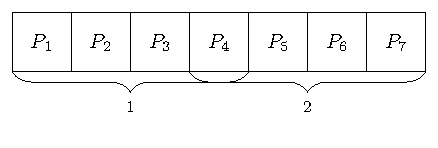
\includegraphics{img/max/filaKernel.pdf}
	\caption{Píxeles contiguos de una fila del kernel, las llaves indican que píxeles se toman en las 2 aplicaciones por fila}
\end{figure}

\begin{center}

	\xmm{1} \xmmDoubleWordSmall{$P_1$}{$P_2$}{$P_3$}{$P_4$}

	\xmm{2} \xmmDoubleWordSmall{$P_5$}{$P_6$}{$P_7$}{$P_8$}

	\texttt{PMAXUB} \xmm{1}, \xmm{2} \hfill

	\xmm{1} \xmmDoubleWordSmall{\tiny$MAX(P_1,P_5)$}{\tiny$MAX(P_2,P_6)$}{\tiny$MAX(P_3,P_7)$}{\tiny$MAX(P_4,P_8)$}

	$MAX(PM,P)$ = \xmmDoubleWordSmall{\tiny$MAX(PM^r,P^r)$}{\tiny$MAX(PM^g,P^g)$}{\tiny$MAX(PM^b,P^b)$}{\tiny$MAX(PM^a,P^a)$}
\end{center}

Una vez realizado esto sobre cada fila, vamos a tener en el registro los cuatro posibles píxeles máximos, ahora debemos compararlos entre sí para conseguir el píxel que contenga el máximo de cada componente. Para esto podemos seguir usando PMAXUB, duplicamos el registro y shifteamos 8 bytes a la derecha uno de ellos, para que nos quede desplazado 2 píxeles y podamos comparar el primer par de píxeles del registro contra el segundo par. Todavía nos queda por comparar 2 píxeles así que repetimos este procedimiento pero esta vez desplazamos un solo píxel, una vez realizado esto nos va a quedar en la parte menos significativa del registro el píxel que estábamos buscando.

\begin{center}
	\xmm{1} \xmmDoubleWordSmall{$M_1$}{$M_2$}{$M_3$}{$M_4$}

	\xmm{2} $\leftarrow$ \xmm{1}

	\texttt{PSRLDQ} \xmm{2}, \texttt{8} \hfill

	\xmm{2} \xmmDoubleWordSmall{0}{0}{$M_1$}{$M_2$}

	\texttt{PMAXUB} \xmm{1}, \xmm{2} \hfill

	\xmm{1} \xmmDoubleWordSmall{$M_1$}{$M_2$}{\tiny$MAX(M_1,M_3)$}{\tiny$MAX(M_2,M_4)$}

	\xmm{2} $\leftarrow$ \xmm{1}

	\texttt{PSRLDQ} \xmm{2}, \texttt{4} \hfill

	\xmm{2} \xmmDoubleWordSmall{0}{$M_1$}{$M_2$}{\tiny$MAX(M_1,M_3)$}

	\texttt{PMAXUB} \xmm{1}, \xmm{2} \hfill

	\xmm{1}
	\vspace{0.1cm}
	\begin{tabular}{|C{1cm}|C{1cm}|C{1cm}|C{3.8cm}|}\hline
		X & X & X & $MAX(M_1,M_2,M_3,M_4)$ \\ \hline
	\end{tabular}
	\vspace{0.1cm}
\end{center}

Ya conseguido el máximo, ahora tenemos que realizar la combinación lineal con el píxel original, el nuevo píxel que generamos y el parámetro. Lo que queremos es hacer la cuenta para cada componente paralelo, para eso, podemos usar instrucciones SIMD para multiplicar las componentes de los píxeles en paralelo por el parámetro, que es un float, entonces convertimos a float cada componente quedándonos todas las componentes en un registro XMM, y para multiplicarlas por el parámetro tenemos que hacer un registro XMM que lo contenga 4 veces y aplicamos MULPS, quedando de resultado la multiplicación por cada componente contra el parámetro cada una en floats. Luego hacemos lo mismo con el píxel original, y sumamos estos dos resultados. Ahora nos queda guardar este resultado en la imagen destino, pero antes, debemos convertir los floats a integers. Ya guardado en memoria, podes seguir repitiendo el paso para los otros píxeles.

\subsection{Análisis preliminar}

\begin{center}
	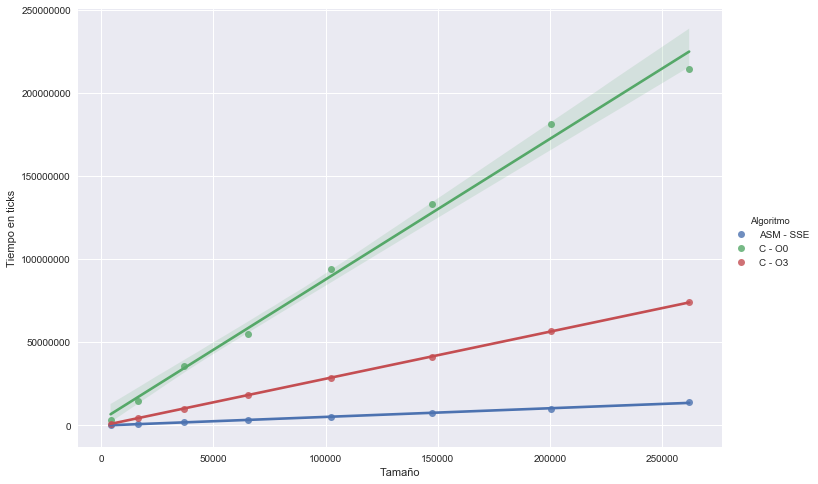
\includegraphics[scale=0.5]{img/maxCloser_CvsASMvsO3.png}
\end{center}

Podemos ver claramente como el filtro implementado en ASM corre más rápido que en C, de hecho, al incrementar el tamaño de la imagen la diferencia es aún más notable. Si bien hay una amplia mejora al compilar con optimizaciones O3, no llega a mejorar la versión de ASM. Es más, la diferencia es la mayor entre todos los filtros estudiados: la implementación en ASM corren en menos de 20\% del tiempo en promedio para una misma imagen.

Esto es un comportamiento esperable ya que en C estamos yendo a buscar el pixel a memoria por cada pixel del kernel, en cambio en ASM con las instrucciones SIMD cada 7 pixeles lo pedimos 2 veces. Además, en ASM aprovechamos y hacemos las cuentas para el pixel destino en paralelo.

\subsection{Experimantación}
Como reveló el análisis preliminar, la cantidad de pixeles origen a procesar por pixel destino tuvo un gran impacto en la performance de nuesto filtro. Decidimos ver cómo impacta en ambas implementaciones si agrandamos el tamaño de kernel. Para esto corrimos los mismos tests que antes, pero ahora con un kernel de 11x11 en vez que de 7x7.

Nuestra hipótesis fue que esta medida afectaría con más contundencia a la implementación de C, si bien en ASM va a tardar más, en relación al kernel mas chico, no le va afectar tanto. Esto es debido a que en C trae cada pixel del kernel uno por vez, y como estamos incrementando el tamaño del kernel en casi 2.5 veces, esperamos una performance peor en este orden. Pero en ASM aprovechando la paralelización de datos, levantamos 11 píxeles con 3 llamadas a memoria nada más.

% TODO: medir esto de nuevo, asegurarse de usar O3, conservar datos en jupyter

\begin{center} 
	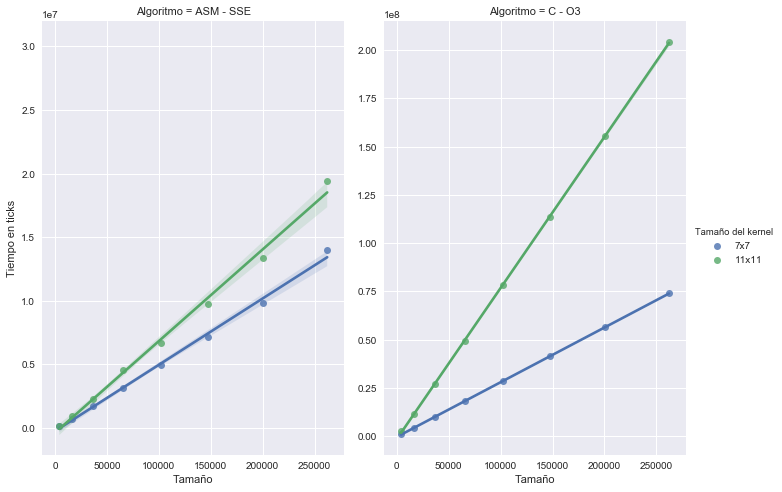
\includegraphics[scale=0.5]{img/maxCloser_KERNEL.png}
	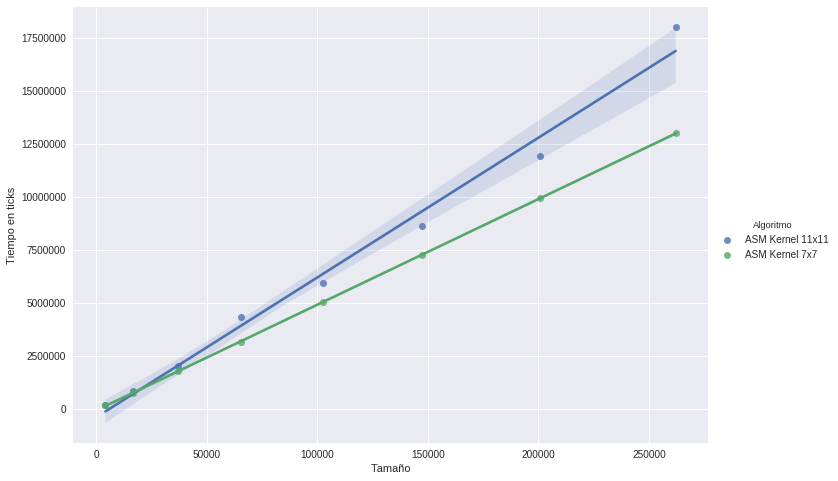
\includegraphics[scale=0.5]{img/maxCloser_KERNEL_ASM.png}
	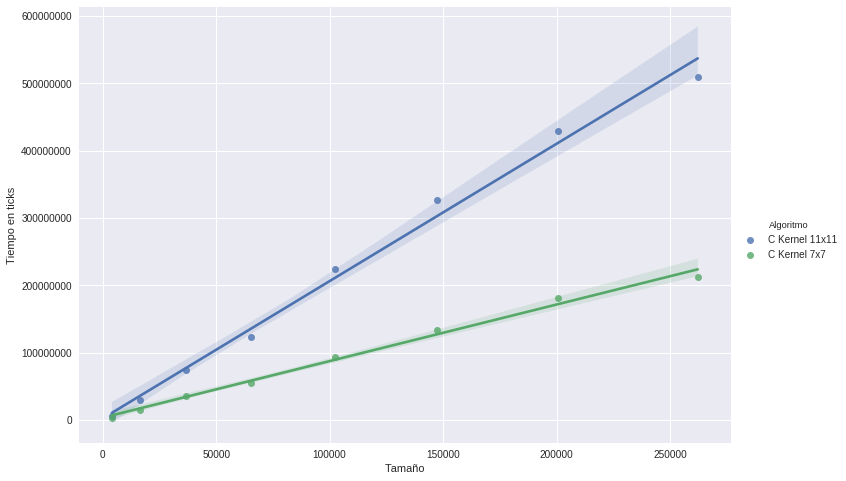
\includegraphics[scale=0.5]{img/maxCloser_KERNEL_C.png}
\end{center}

Si observamos los gráficos, podemos ver como en C con el kernel de 11x11 tarda casi 2.5 veces más, como la relación de diferencia de pixeles en los kernels, y para ASM hay nada mas una diferencia de 1.2 y 1.4 para instancias más grandes. Como habíamos predicho en la hipótesis, este cambio en el tamaño del kernel afectó bastante más a la implementación de C que a la de ASM.

